%!TEX root = Main.tex
\section{Tests}
This section contains the description of the tests done as part of the mini project.

\subsection{Functionality test}

\fxnote{Tests should contain an "expected result" section.}

\subsubsection{Compression}

\textbf{Purpose}\\
The purpose is to validate the compression and decompression method of each compression algorithm.

\textbf{Test equipment}
\begin{itemize}
\item PC 
\item TelosB mote
\end{itemize}

\textbf{Procedure}
\begin{enumerate}
\item Connect the TelosB mote to the PC.
\item Load a compression module on the mote.
\item Open a terminal and connect the output from the mote to the terminal with the command \texttt{java net.tinyos.tools.PrintfClient -comm serial@/dev/ttyUSB0:telos}
\item Press the RESET button on the mote.
\item Observe data in the terminal.
\item Repeat step 2 to 5 for every compression module.
\end{enumerate}

\subsubsection{Full System Test}
\label{subs:FST}
\textbf{Purpose}\\
The purpose is to validate the full system functionality.

\textbf{Test equipment}
\begin{itemize}
\item PC with TestSerial Java software
\item Receiver TelosB mote
\item Sender TelosB mote
\end{itemize}
The compressed images can be seen on figure \ref{fig:cameramanresult}. 
To ensure that the compression-send-decompress procedure was successful it is compared with the same image compressed and decompressed in Matlab. 
By comparing this two images it is shown that the functionality is as expected. 

\textbf{Procedure}
\begin{enumerate}
\item Connect the Sender TelosB mote to the PC.
\item Load the image onto the sender TelosB using the command: \texttt{Java TestSerial -w}.
\item When the transfer to the Sender TelosB mote is complete, reset the mote. 
\item When the transmission is complete, connect the Receiver TelosB mote to the PC and execute the terminal command: \texttt{Java TestSerial -r}. \\
(LED2 on the Receiver mote will light up when the wireless transmission is completed.)
\item Observe the reconstructed image on the PC.
\end{enumerate}

Looking at the voltage over the shunt, we can see how the system uses power, for the test setup a typical power over time is illustrated in Figure \ref{fig:ImageTransfere}.

\subsection{Energy Test}
\textbf{Purpose} \\
The purpose is to validate the energy consumption of the full system functionality.

\textbf{Test equipment}
\begin{itemize}
\item PC with TestSerial Java software
\item Receiver TelosB mote
\item Sender TelosB mote
\item Oscilloscope
\item 10 Ohm shunt resistor board
\end{itemize}
For each compression algorithm 3 measurements was done on both sender and receiver. The measurements can be seen in the table \ref{tab:MeasurementResults}.

\textbf{Procedure}
\begin{enumerate}
\item Choose a compression module on the two TelosB motes.
\item Connect the Sender TelosB mote to the PC.
\item Load the image onto the sender TelosB using the terminal command: \texttt{Java TestSerial -w}.
\item When the transfer to the Sender TelosB mote is complete, set the oscilloscope to single mode and reset the mote.
\item When the wireless transmission is complete, observe and save the reading from the oscilloscope. \\
(LED2 on the Receiver mote will light up when the wireless transmission is completed.)
\item Connect the Receiver TelosB mote to the PC and execute the terminal command: \texttt{Java TestSerial -r}.
\item Observe the reconstructed image on the PC.
\end{enumerate}

\section{Results}
This section contains the results of the tests done during the mini project.

Before the energy measurements are made, the functionality was validated. Using the test setup in section \ref{subs:FST}, an image was written to the flash, and then compressed and sent. 

\begin{figure}[H]
	\centering
	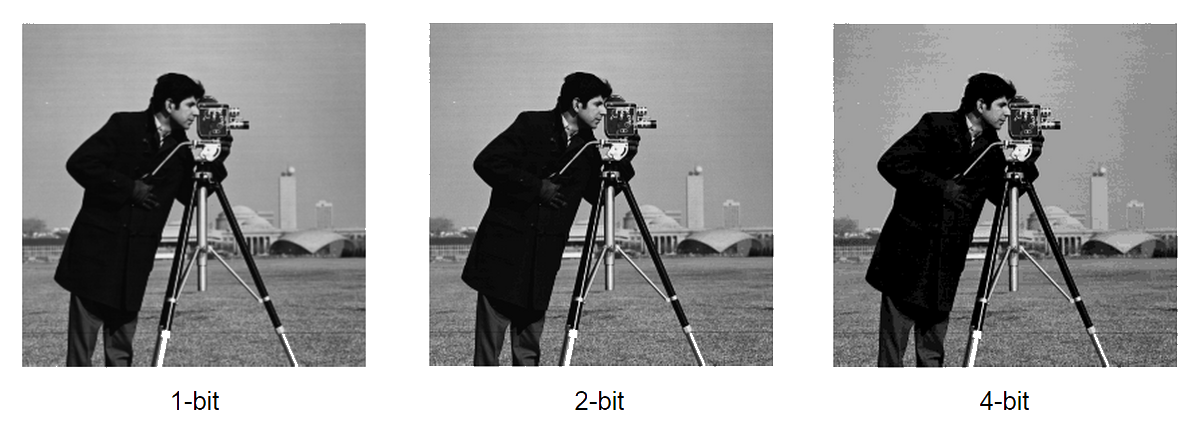
\includegraphics[width=0.8\textwidth] {cameramanresult}
	\caption{Compression Results}
	\label{fig:cameramanresult}
\end{figure}

The compressed images can be seen on figure \ref{fig:cameramanresult}. To ensure that the compression-send-decompress procedure was successful it is compared with the same image compressed and decompressed in Matlab. By comparing this two images it is shown that the functionality is as expected. 


Looking at the voltage over the shunt, we can see how the system uses power, for the test setup a typical power over time is illustrated in figure \ref{fig:ImageTransfere}

\begin{figure}[H]
	\centering
	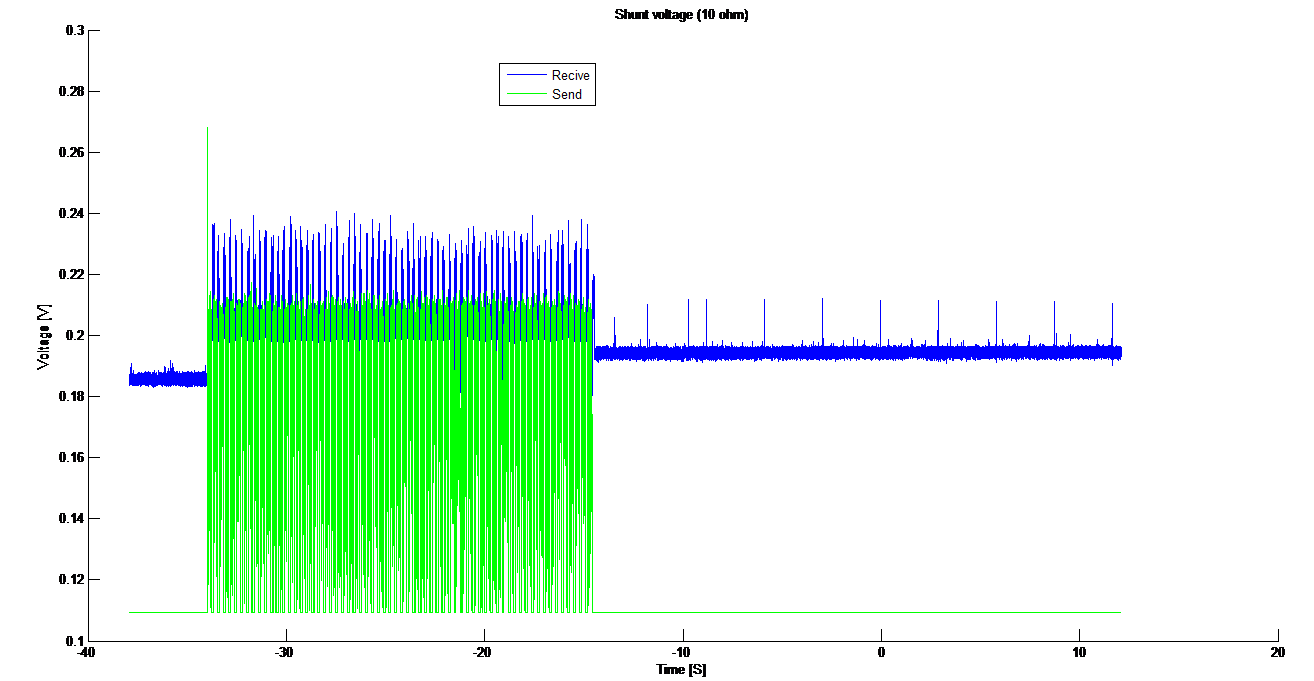
\includegraphics[width=1\textwidth ]{ImageTransfere}
	\caption{ Shut voltage during image transfer. }
	\label{fig:ImageTransfere}
\end{figure}

For each compression algorithm 3 measurements was done on both sender and receiver. The measurements can be seen in the table \ref{tab:MeasurementResults} 


\begin{table}[h]
	\begin{tabular}{cllllll}

	\cline{2-5} 
	\multicolumn{1}{l}{} 	& \multicolumn{2}{l}{Energy {[$J$]}} & \multicolumn{2}{l}{Mean Power [$W$]} &	&	\\ \hline
	\rowcolor{gr}
	\multicolumn{1}{l}{Bit Removed}	& Recive	& Send	& Recive	& Sender	& \multicolumn{1}{l}{Transfer Time [$S$]} & \multicolumn{1}{l}{Better Power Than None} \\ \hline
	% \rowcolor{gr}
	\multicolumn{1}{c}{\multirow{3}{*}{None}} & 14,638	& 14,405	& 0,639	& 0,626	& \multicolumn{1}{l}{23,0}	& \multicolumn{1}{l}{0\%}	\\  
	\multicolumn{1}{c}{}	& 14,666	& 14,432	& 0,639	& 0,626	& \multicolumn{1}{l}{23,0}	& \multicolumn{1}{l}{0\%}	\\ 
	% \rowcolor{gr} 
	\multicolumn{1}{c}{}	& 14,609	& 14,385	& 0,639	& 0,626	& \multicolumn{1}{l}{23,0}	& \multicolumn{1}{l}{0\%}	\\ \hline
	% \rowcolor{gr} 
	\multicolumn{1}{c}{\multirow{3}{*}{One}}  & 13,527	& 13,248	& 0,642	& 0,625	& \multicolumn{1}{l}{21,2}	& \multicolumn{1}{l}{8\%}	\\ %\cline{2-7} 
	\multicolumn{1}{c}{}	& 13,535	& 13,252	& 0,642	& 0,626	& \multicolumn{1}{l}{21,2}	& \multicolumn{1}{l}{8\%}	\\ %\cline{2-7} 
	% \rowcolor{gr} 
	\multicolumn{1}{c}{}	& 13,528	& 13,254	& 0,642	& 0,625	& \multicolumn{1}{l}{21,2}	& \multicolumn{1}{l}{8\%}	\\ \hline
	% \rowcolor{gr} 
	\multicolumn{1}{c}{\multirow{3}{*}{Two}}  & 12,469	& 12,189	& 0,643	& 0,625	& \multicolumn{1}{l}{19,5}	& \multicolumn{1}{l}{15\%}	\\ %\cline{2-7} 
	\multicolumn{1}{c}{}	& 12,477	& 12,206	& 0,643	& 0,626	& \multicolumn{1}{l}{19,5}	& \multicolumn{1}{l}{15\%}	\\ %\cline{2-7} 
	% \rowcolor{gr}
	\multicolumn{1}{c}{}	& 12,467	& 12,190	& 0,643	& 0,625	& \multicolumn{1}{l}{19,5}	& \multicolumn{1}{l}{15\%}	\\ \hline
	% \rowcolor{gr}
	\multicolumn{1}{c}{\multirow{3}{*}{Four}} & 9,566	& 9,317	& 0,646	& 0,624	& \multicolumn{1}{l}{14,9}	& \multicolumn{1}{l}{35\%}	\\ %\cline{2-7} 
	\multicolumn{1}{c}{}	& 9,556	& 9,309	& 0,646	& 0,625	& \multicolumn{1}{l}{14,9}	& \multicolumn{1}{l}{35\%}	\\ %\cline{2-7} 
	% \rowcolor{gr}
	\multicolumn{1}{c}{}	& 9,533	& 9,298	& 0,644	& 0,625	& \multicolumn{1}{l}{14,9}	& \multicolumn{1}{l}{35\%}	\\ \hline
	\end{tabular}

	\caption{Measurement Results }
	\label{tab:MeasurementResults}
\end{table}
